\documentclass[12pt,letterpaper]{article}
\usepackage{graphicx,textcomp}
\usepackage{natbib}
\usepackage{setspace}
\usepackage{fullpage}
\usepackage{color}
\usepackage[reqno]{amsmath}
\usepackage{amsthm}
\usepackage{fancyvrb}
\usepackage{amssymb,enumerate}
\usepackage[all]{xy}
\usepackage{endnotes}
\usepackage{lscape}
\newtheorem{com}{Comment}
\usepackage{float}
\usepackage{hyperref}
\newtheorem{lem} {Lemma}
\newtheorem{prop}{Proposition}
\newtheorem{thm}{Theorem}
\newtheorem{defn}{Definition}
\newtheorem{cor}{Corollary}
\newtheorem{obs}{Observation}
\usepackage[compact]{titlesec}
\usepackage{dcolumn}
\usepackage{tikz}
\usetikzlibrary{arrows}
\usepackage{multirow}
\usepackage{xcolor}
\newcolumntype{.}{D{.}{.}{-1}}
\newcolumntype{d}[1]{D{.}{.}{#1}}
\definecolor{light-gray}{gray}{0.65}
\usepackage{url}
\usepackage{listings}
\usepackage{color}

\definecolor{codegreen}{rgb}{0,0.6,0}
\definecolor{codegray}{rgb}{0.5,0.5,0.5}
\definecolor{codepurple}{rgb}{0.58,0,0.82}
\definecolor{backcolour}{rgb}{0.95,0.95,0.92}

\lstdefinestyle{mystyle}{
	backgroundcolor=\color{backcolour},   
	commentstyle=\color{codegreen},
	keywordstyle=\color{magenta},
	numberstyle=\tiny\color{codegray},
	stringstyle=\color{codepurple},
	basicstyle=\footnotesize,
	breakatwhitespace=false,         
	breaklines=true,                 
	captionpos=b,                    
	keepspaces=true,                 
	numbers=left,                    
	numbersep=5pt,                  
	showspaces=false,                
	showstringspaces=false,
	showtabs=false,                  
	tabsize=2
}
\lstset{style=mystyle}
\newcommand{\Sref}[1]{Section~\ref{#1}}
\newtheorem{hyp}{Hypothesis}

\title{Problem Set 1}
\date{Due: September 30, 2024}
\author{Applied Stats/Quant Methods 1
\\ Jianxiong Wu---23354731}

\begin{document}
	\maketitle
	
	\section*{Instructions}
	\begin{itemize}
	\item Please show your work! You may lose points by simply writing in the answer. If the problem requires you to execute commands in \texttt{R}, please include the code you used to get your answers. Please also include the \texttt{.R} file that contains your code. If you are not sure if work needs to be shown for a particular problem, please ask.
\item Your homework should be submitted electronically on GitHub.
\item This problem set is due before 23:59 on Monday September 30, 2024. No late assignments will be accepted.
%\item Total available points for this homework is 80.
	\end{itemize}
	
	\vspace{1cm}
	\section*{Question 1: Education}

A school counselor was curious about the average of IQ of the students in her school and took a random sample of 25 students' IQ scores. The following is the data set:\\
\vspace{.5cm}

\lstinputlisting[language=R, firstline=38, lastline=38]{PS01_Jianxiong Wu_23354731.R}  

\vspace{1cm}

\begin{enumerate}
	\item Find a 90\% confidence interval for the average student IQ in the school.\\
	
	\lstinputlisting[language=R, firstline=38, lastline=39]{PS01_Jianxiong Wu_23354731.R}  
	
	\begin{verbatim} 
		Results: 
		data:  y
		t = 37.593, df = 24, p-value < 2.2e-16
		alternative hypothesis: true mean is not equal to 0
		90 percent confidence interval:
		93.95993 102.92007
		sample estimates:
		mean of x 
		98.44 
		
		Answer: 90 percent confidence interval:93.95993 102.92007
	\end{verbatim}
	
	
	\item Next, the school counselor was curious  whether  the average student IQ in her school is higher than the average IQ score (100) among all the schools in the country.\\ 
	
	\noindent Using the same sample, conduct the appropriate hypothesis test with $\alpha=0.05$.
	
	\lstinputlisting[language=R, firstline=41, lastline=41]{PS01_Jianxiong Wu_23354731.R}  
	
	\begin{verbatim} 
		Results:
		data:  y
		t = -0.59574, df = 24, p-value = 0.7215
		alternative hypothesis: true mean is greater than 100
		95 percent confidence interval:
		93.95993      Inf
		sample estimates:
		mean of x 
		98.44 
		
		Answer: p-value = 0.7215, p-value > 0.05, so there is not sufficient 
		evidence to suggest that the average student IQ in school is higher 
		than the average IQ score (100) among all the schools in the country.
	\end{verbatim}
	
	
\end{enumerate}

\newpage

	\section*{Question 2: Political Economy}

\noindent Researchers are curious about what affects the amount of money communities spend on addressing homelessness. The following variables constitute our data set about social welfare expenditures in the USA. \\
\vspace{.5cm}


\begin{tabular}{r|l}
	\texttt{State} &\emph{50 states in US} \\
	\texttt{Y} & \emph{per capita expenditure on shelters/housing assistance in state}\\
	\texttt{X1} &\emph{per capita personal income in state} \\
	\texttt{X2} &  \emph{Number of residents per 100,000 that are "financially insecure" in state}\\
	\texttt{X3} &  \emph{Number of people per thousand residing in urban areas in state} \\
	\texttt{Region} &  \emph{1=Northeast, 2= North Central, 3= South, 4=West} \\
\end{tabular}

\vspace{.5cm}
\noindent Explore the \texttt{expenditure} data set and import data into \texttt{R}.
\vspace{.5cm}
\begin{itemize}

\item
Please plot the relationships among \emph{Y}, \emph{X1}, \emph{X2}, and \emph{X3}? What are the correlations among them (you just need to describe the graph and the relationships among them)?
\vspace{.5cm}

\lstinputlisting[language=R, firstline=53, lastline=95]{PS01_Jianxiong Wu_23354731.R}  



\begin{figure}[h!]\centering
	\caption{\footnotesize X1 and Y}
	\label{fig:plot_1}
	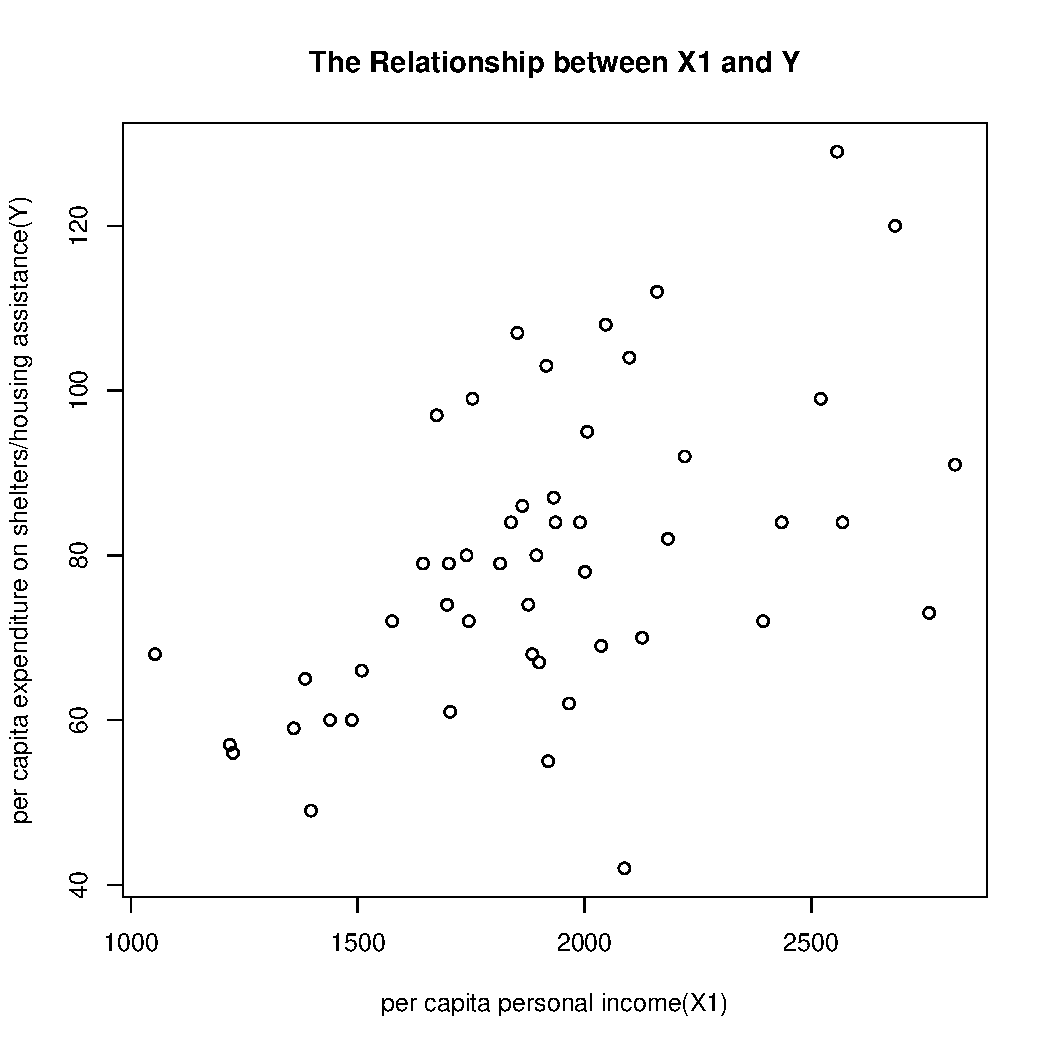
\includegraphics[width=.75\textwidth]{scatter_plot1_X1&Y.pdf}
\end{figure}
\newpage
\begin{verbatim} 
	Results: Figure 1 shows that the correlation coefficient between X1 and Y 
	is 0.5317212, indicating a positive correlation.
\end{verbatim}

\newpage
\begin{figure}[h!]\centering
	\caption{\footnotesize X2 and Y}
	\label{fig:plot_2}
	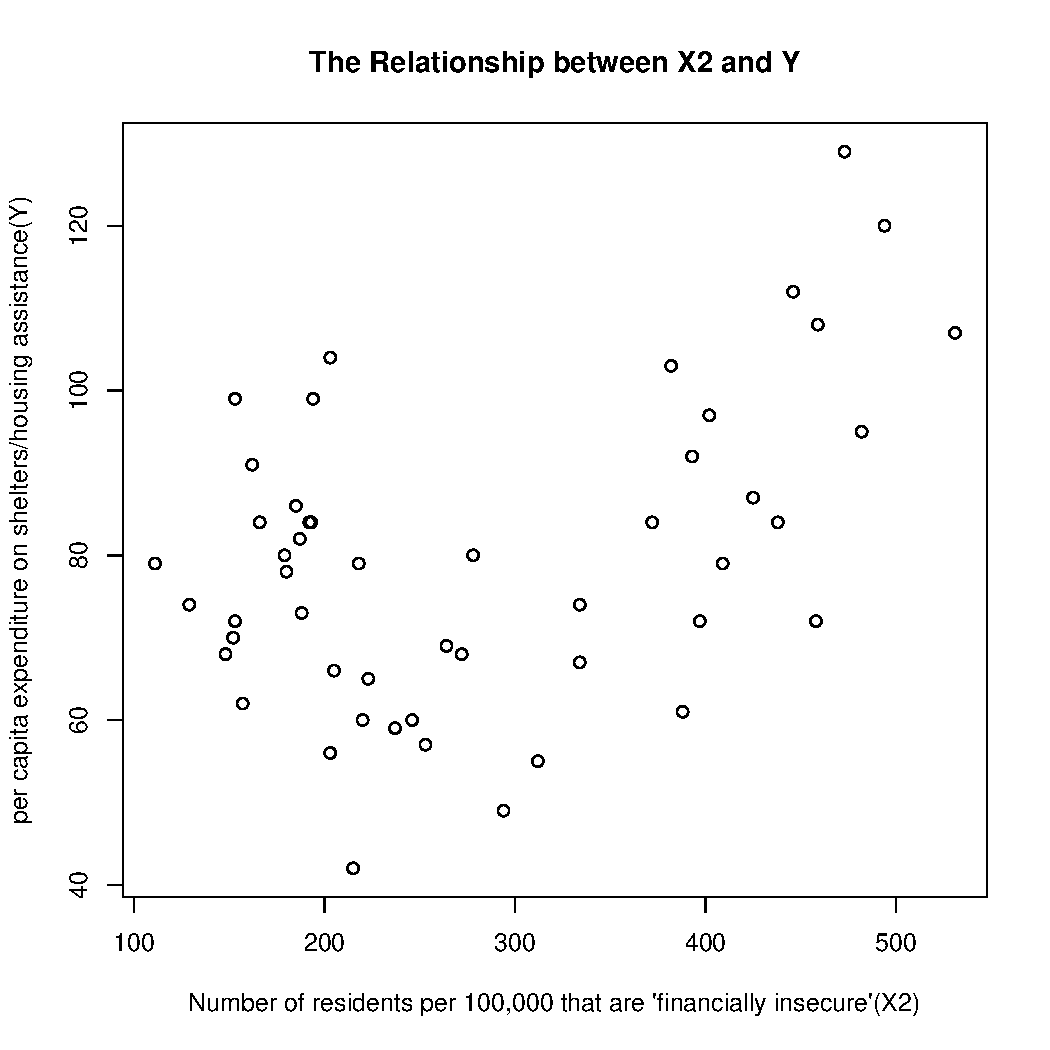
\includegraphics[width=.75\textwidth]{scatter_plot2_X2&Y.pdf}
\end{figure}

\begin{verbatim} 
	Results: Figure 2 shows that the correlation coefficient between X2 and Y 
	is 0.4482876, indicating a positive correlation.
\end{verbatim}

\newpage
\begin{figure}[h!]\centering
	\caption{\footnotesize X3 and Y}
	\label{fig:plot_3}
	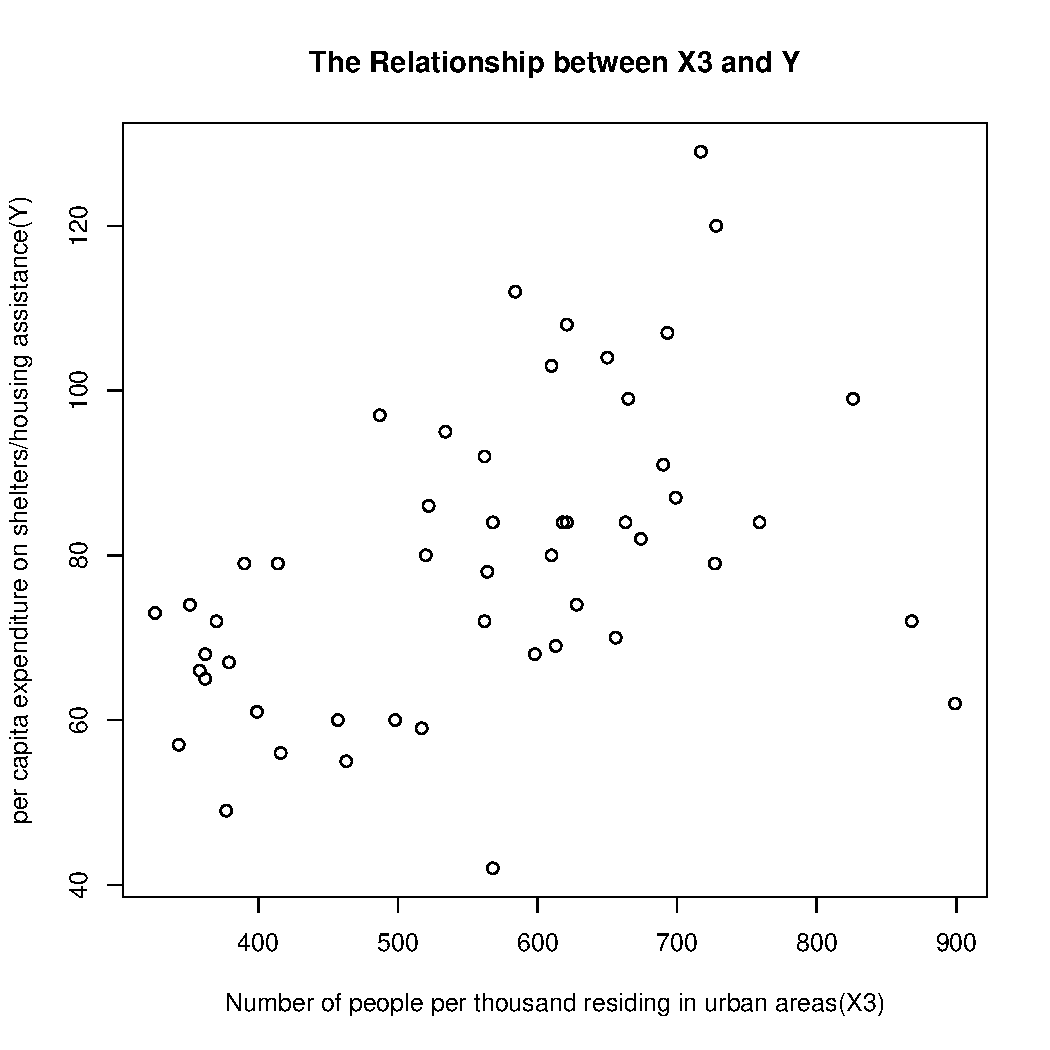
\includegraphics[width=.75\textwidth]{scatter_plot3_X3&Y.pdf}
\end{figure}

\begin{verbatim} 
	Results: Figure 3 shows that the correlation coefficient between X3 and Y 
	is 0.4636787, indicating a positive correlation.
\end{verbatim}

\newpage
\begin{figure}[h!]\centering
	\caption{\footnotesize X1 and X2}
	\label{fig:plot_4}
	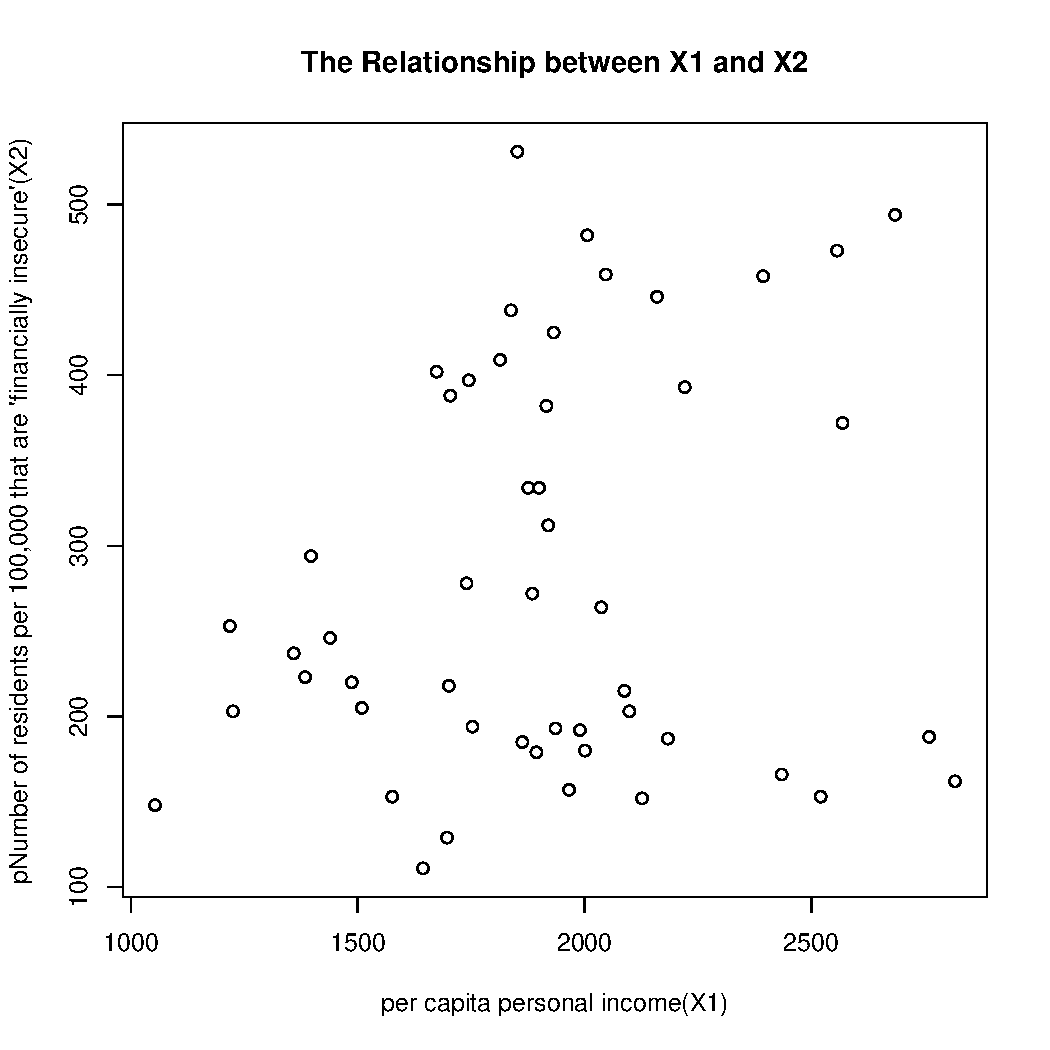
\includegraphics[width=.75\textwidth]{scatter_plot4_X1&X2.pdf}
\end{figure}

\begin{verbatim} 
	Results: Figure 4 shows that the correlation coefficient between X1 and X2 
	is 0.2056101, indicating a positive correlation, but this relationship is 
	relatively weak.
\end{verbatim}

\newpage
\begin{figure}[h!]\centering
	\caption{\footnotesize X1 and X3}
	\label{fig:plot_5}
	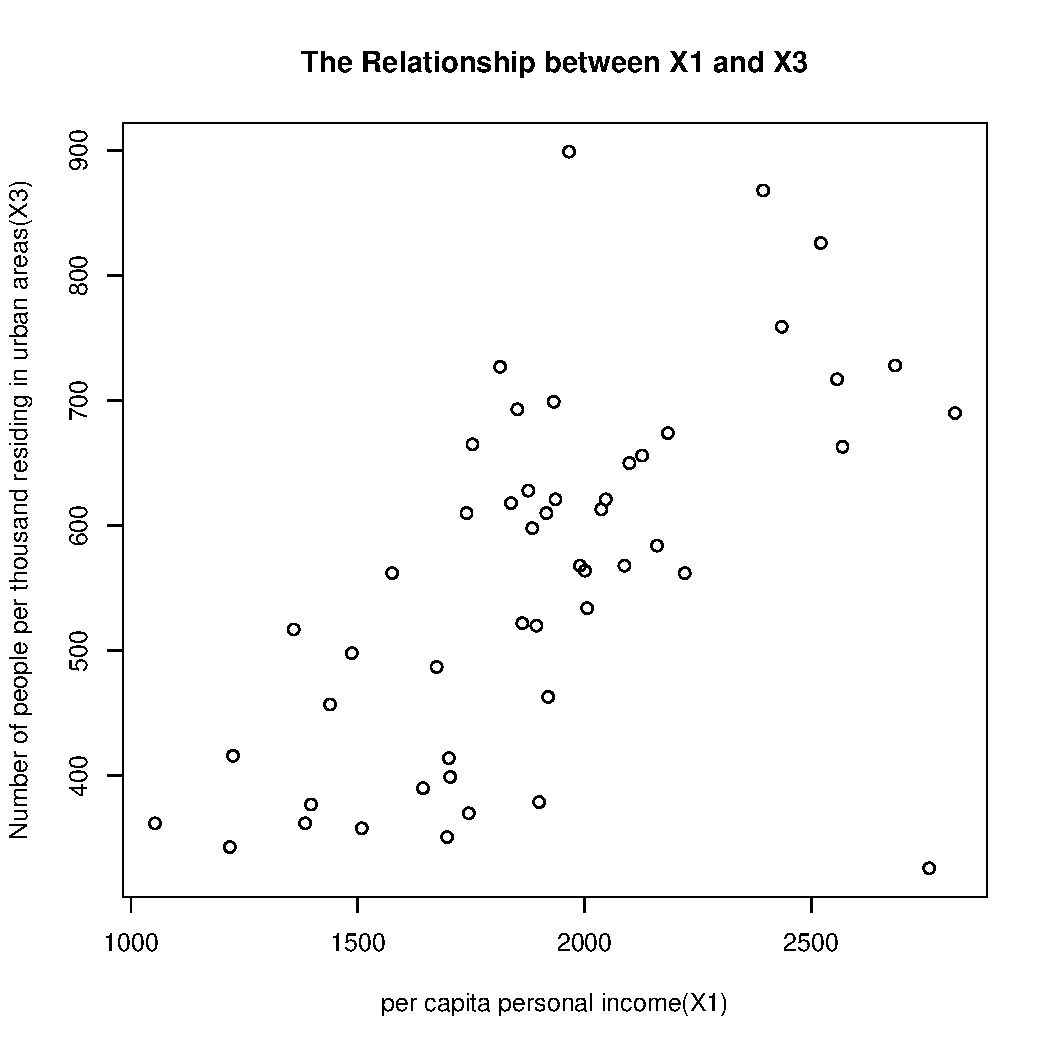
\includegraphics[width=.75\textwidth]{scatter_plot5_X1&X3.pdf}
\end{figure}

\begin{verbatim} 
	Results: Figure 5 shows that the correlation coefficient between X1 and X3 
	is 0.5952504, indicating a positive correlation.
\end{verbatim}

\newpage
\begin{figure}[h!]\centering
	\caption{\footnotesize X2 and X3}
	\label{fig:plot_6}
	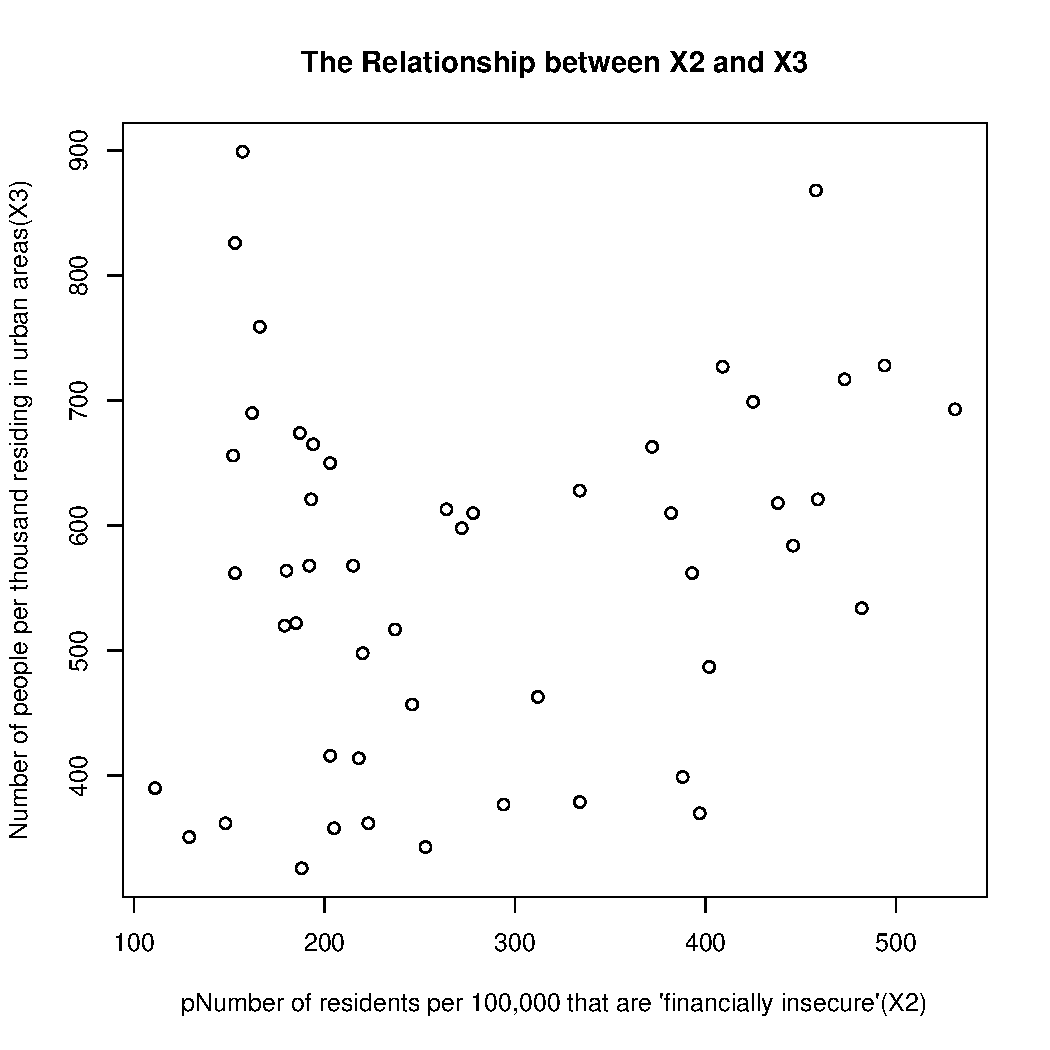
\includegraphics[width=.75\textwidth]{scatter_plot6_X2&X3.pdf}
\end{figure}

\begin{verbatim} 
	Results: Figure 6 shows that the correlation coefficient between X2 and X3 
	is 0.2210149, indicating a positive correlation, but this relationship is 
	relatively weak.
\end{verbatim}

\newpage
\begin{verbatim} 
    Results: 
               Y        X1        X2        X3
    Y  1.0000000 0.5317212 0.4482876 0.4636787
    X1 0.5317212 1.0000000 0.2056101 0.5952504
    X2 0.4482876 0.2056101 1.0000000 0.2210149
    X3 0.4636787 0.5952504 0.2210149 1.0000000
    
    Answer: 
    The results show that the relationships between Y, X1, X2 and X3 are all 
    positively correlated.The correlation coefficient between X1 and X3 is 
    0.5952504 and between X1 and Y is 0.5317212, which indicates that the 
    positive relationship between these two groups is relatively strong among 
    all the data.While the correlation coefficient between X1 and X2 is 
    0.2056101 and between X2 and X3 is 0.2210149, indicating that the 
    positive relationship between these two groups of data is relatively weak.
\end{verbatim}

\vspace{.5cm}
\item
Please plot the relationship between \emph{Y} and \emph{Region}? On average, which region has the highest per capita expenditure on housing assistance?
\vspace{.5cm}

\lstinputlisting[language=R, firstline=99, lastline=105]{PS01_Jianxiong Wu_23354731.R}  

\begin{figure}[h!]\centering
	\caption{\footnotesize Y and Region}
	\label{fig:plot_7}
	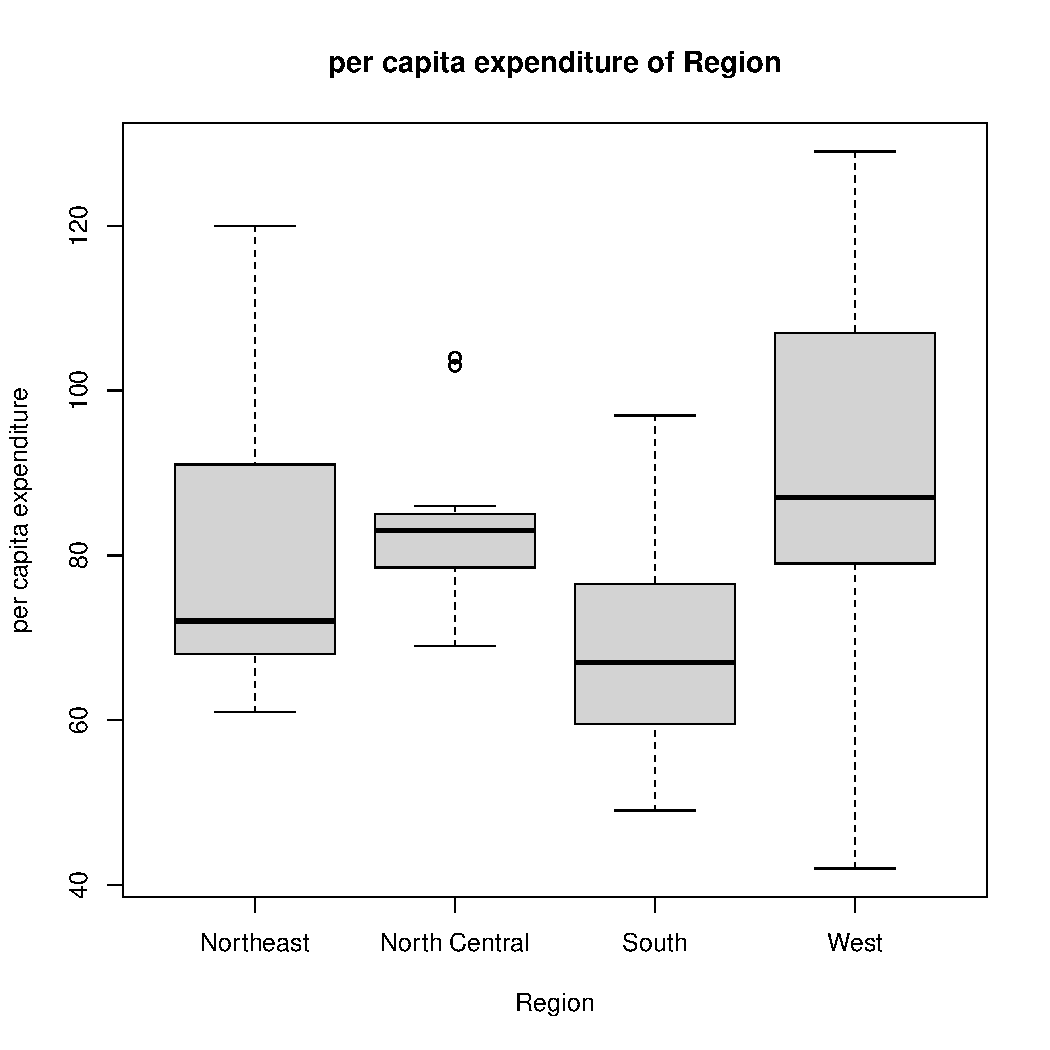
\includegraphics[width=.75\textwidth]{boxplot_plot7_Y&Region.pdf}
\end{figure}

\newpage
\begin{verbatim} 
	Answer: Figure 7 shows that, region West has the highest per capita 
	expenditure on housing assistance.
\end{verbatim}

\vspace{.5cm}
\item
Please plot the relationship between \emph{Y} and \emph{X1}? Describe this graph and the relationship. Reproduce the above graph including one more variable \emph{Region} and display different regions with different types of symbols and colors.
\end{itemize}
\vspace{.5cm}

\lstinputlisting[language=R, firstline=111, lastline=121]{PS01_Jianxiong Wu_23354731.R}  

\begin{figure}[h!]\centering
	\caption{\footnotesize Y and X1(Region)}
	\label{fig:plot_8}
	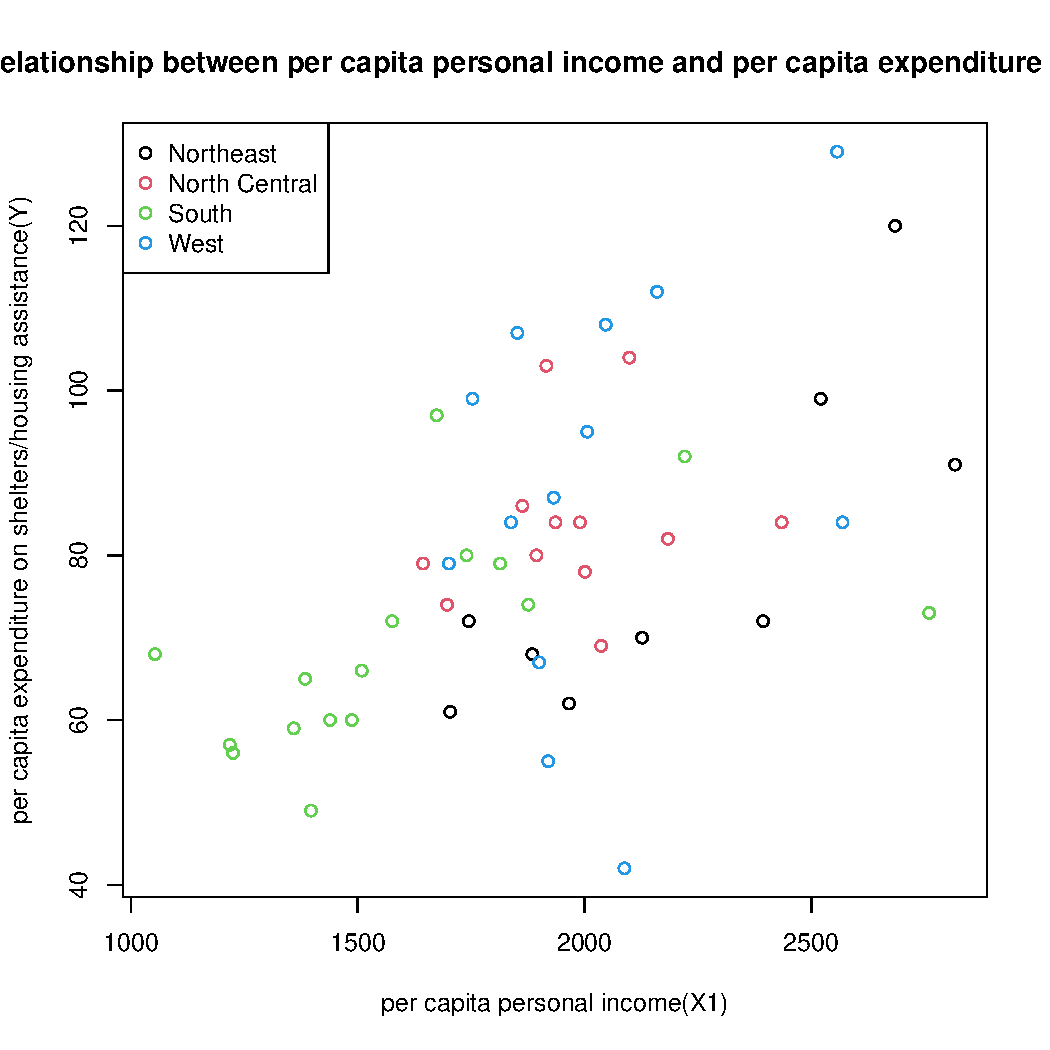
\includegraphics[width=.75\textwidth]{scatter_plot8_X1&Y_Region.pdf}
\end{figure}
\begin{verbatim} 
	Answer: Figure 8 shows that there is a positive correlation between Y and X1 
	in all regions, suggesting that as per capita personal income increases, per 
	capita expenditure on shelters/housing assistance also increase. The positive 
	correlation is stronger in the Northeast and South regions, while the correlation 
	is weaker in the North Central and West regions.
\end{verbatim}



\end{document}
